\documentclass{beamer}
\usepackage{tcolorbox}
\usepackage{caption}

\usetheme{szeged}
\usecolortheme{beaver}
\usepackage{graphicx}
 
\title{DS289 NSDE Project - ODE Module \\
        Group - 01 \\
        Chemical kinetics of hydrogen combustion }

\author{Aswin Kumar A \and 
        Deepti Sahu \and
        Surya Datta Sudhakar}
\institute{CDS, Indian Institute of Science}
\date{January 31, 2025}

\begin{document}
\begin{frame}
\maketitle
\end{frame}

%%%%%%%%%%%%%%%%%%%%%%%%%%%%%%%%%%%%%%%%%%%%%%%%%%%%%%%%%%%%%%%%%%%%%%%
%%%%%%%%%%%%%%%%%%%%%%%%%%%%%%%%%%%%%%%%%%%%%%%%%%%%%%%%%%%%%%%%%%%%%%%

\begin{frame}{Governing Equations}
\begin{itemize}
    % \item Hydrogen combustion
    \item Detailed chemical kinetics by Li\footnote{J. Li et al., 
    \textit{An updated comprehensive kinetic model of hydrogen combustion}, 
    IJCK, 2004} 
    with 9 species and 21 reactions
    \item Species: $ H_2, H, O_2, O, OH, HO_2, H_2O, H_2O_2, N_2 $
\end{itemize}

\begin{tcolorbox}[width=0.5\linewidth,center,colback=blue!15!white]
\begin{equation*}
    \dfrac{d X_k}{dt} = \dfrac{W}{\rho} \dot{\omega}_k
\end{equation*}
\end{tcolorbox}

\begin{equation*}
    \text{where } k=1, \ldots, N_s
\end{equation*}

\vspace*{-4mm}
% \begin{equation*}
%     \dot{\omega}_k = \sum_{j=1}^{N_R} \kappa_{kj} \prod_{i=1}^{N_s} [R_i]^{\mu_{ij}}
% \end{equation*}
\begin{center}
    $ \dot{\omega}_k $ : net production rate of species $ k $
\end{center}


\end{frame}

%%%%%%%%%%%%%%%%%%%%%%%%%%%%%%%%%%%%%%%%%%%%%%%%%%%%%%%%%%%%%%%%%%%%%%%
%%%%%%%%%%%%%%%%%%%%%%%%%%%%%%%%%%%%%%%%%%%%%%%%%%%%%%%%%%%%%%%%%%%%%%%


\begin{frame}{Objectives}
\textbf{Assigned Objectives}:
\begin{itemize}
    \item Use of adaptive time stepping (explicit schemes)
    \item Effect of precision on capturing physics
\end{itemize}

\vspace*{4mm}
\textbf{Exploratory Objectives}:
\begin{itemize}
    \item Studying effect of free parameters like tolerance
    \item Computational time vs Accuracy by varying the local error term
    using two different reference schemes
    \item Exploring implicit adaptive time stepping
\end{itemize}
\end{frame}


%%%%%%%%%%%%%%%%%%%%%%%%%%%%%%%%%%%%%%%%%%%%%%%%%%%%%%%%%%%%%%%%%%%%%%%
%%%%%%%%%%%%%%%%%%%%%%%%%%%%%%%%%%%%%%%%%%%%%%%%%%%%%%%%%%%%%%%%%%%%%%%

\begin{frame}{Methodology}
\begin{itemize}
    \item Determine $ \Delta t $ based on local error
    \item \textbf{Schemes}
    \begin{enumerate}
        \item Main scheme: Lower order
        \item "Reference" scheme: Higher order
    \end{enumerate}
    \item \textbf{Performance / Analysis metrics}
    \begin{enumerate}
        \item $\Delta t_{min}$ for adaptive time stepping
        \item Use of $\Delta t_{min}$ as constant time step (comparison metric)
        \item Effect of precision (double vs single vs half) on auto-ignition problem by comparing
        \begin{enumerate}
            \item Ignition delay time
            \item Minor species evolution
        \end{enumerate}
    \end{enumerate}
    \item \textbf{Programming language}
    \begin{itemize}
        \item Python (cantera library for chemical kinetics)
    \end{itemize}
    \item \textbf{LLM tools}
    \begin{itemize}
        \item ChatGPT, Copilot, Gemini, DeepSeek
    \end{itemize}
\end{itemize}
\end{frame}

%%%%%%%%%%%%%%%%%%%%%%%%%%%%%%%%%%%%%%%%%%%%%%%%%%%%%%%%%%%%%%%%%%%%%%%
%%%%%%%%%%%%%%%%%%%%%%%%%%%%%%%%%%%%%%%%%%%%%%%%%%%%%%%%%%%%%%%%%%%%%%%

\begin{frame}{Expected Outcomes}
    \begin{columns}
        \begin{column}{0.5\textwidth}
            \begin{figure}[h!]
                \captionsetup{labelformat=empty, labelsep=none, justification=centering}
                \centering
                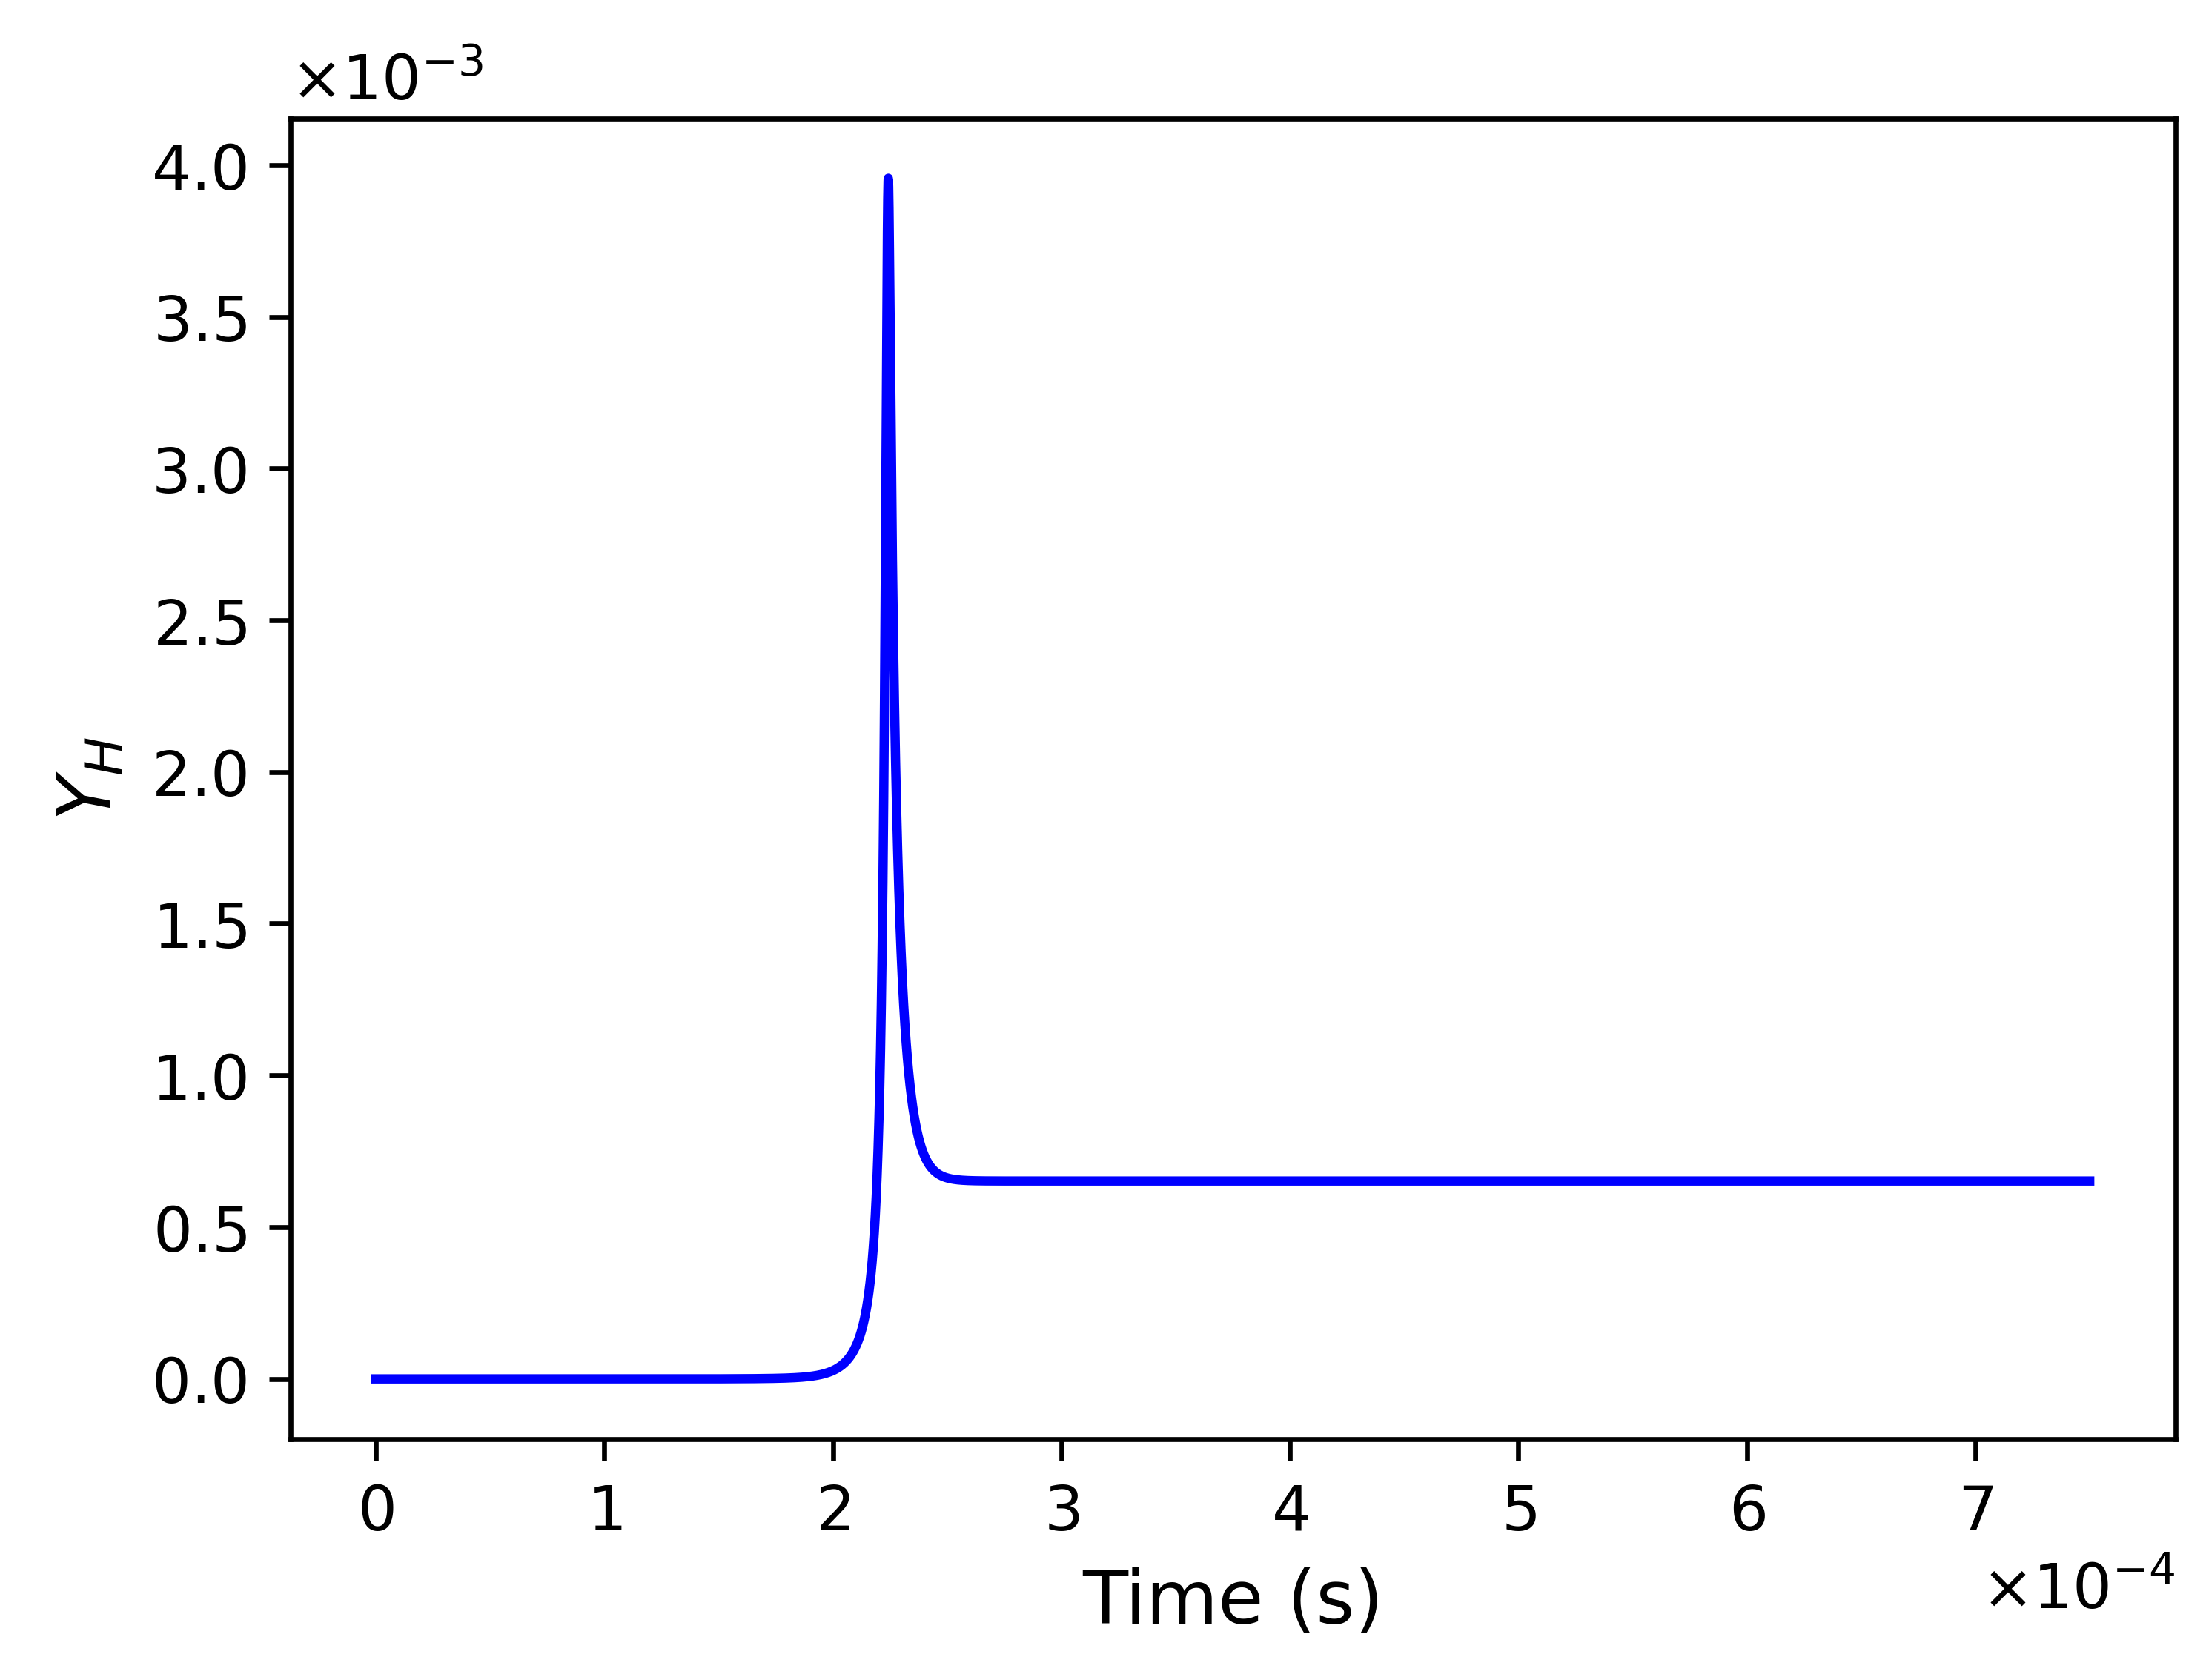
\includegraphics[width=\textwidth]{D:/actual files in this 2/to_sort/nsde/project01/YH1.png}
                \vspace*{-3mm}
                \caption{}
                \label{fig01}
            \end{figure}
        \end{column}

        \begin{column}{0.5\textwidth}
            \begin{figure}[h!]
                \captionsetup{labelformat=empty, labelsep=none, justification=centering}
                \centering
                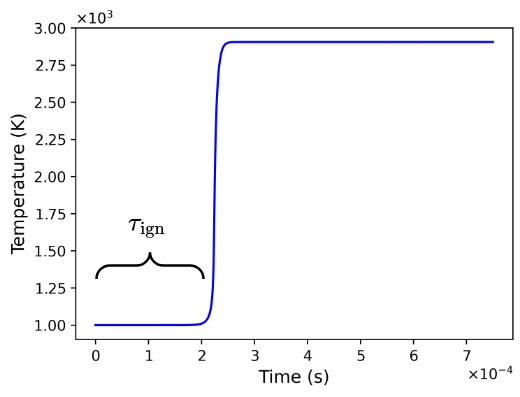
\includegraphics[width=\textwidth]{D:/actual files in this 2/to_sort/nsde/project01/T2.png}
                \vspace*{-3mm}
                \caption{}
                \label{fig02}
            \end{figure}
        \end{column}
    \end{columns}
\vspace*{-1cm}
\begin{itemize}
    \item Adaptive time stepping expected to be faster than traditional solver
    \item Sensitive quantities are expected to be affected by precision
\end{itemize}
\vspace*{3mm}
\tiny
\raggedright
\noindent
Plots generated with cantera constant volume reactor
\end{frame}


%%%%%%%%%%%%%%%%%%%%%%%%%%%%%%%%%%%%%%%%%%%%%%%%%%%%%%%%%%%%%%%%%%%%%%%
%%%%%%%%%%%%%%%%%%%%%%%%%%%%%%%%%%%%%%%%%%%%%%%%%%%%%%%%%%%%%%%%%%%%%%%


\end{document}